\section{Method}
\label{method}
%\textcolor{red}{add some hypotheses about how beta should behave, and whether it's rational to think that it should be stable over time for one category}
We present a comprehensive method to {\it reverse-engineer} coordination as a feature of categories in Wikipedia.  We expect that categories of articles exhibit more or less coordination, which in turn can be captured by the fundamental structure of the {\it bi-partite} network of articles and editors. The underlying idea of our model is to account for the recursive flow of {\it value} circulating between editors and articles, with editors benefiting from having edited higher quality articles, and articles having been edited by more expert editors. If coordination brings ``more than the sum of its parts", then articles benefit from more editors, and primarily from expert editors. Conversely, if coordination is not efficient, {\it disvalue} is generated by more editors editing one article, or by an editor contributing to many articles in the category. A typical example of disvalue is vandalism \cite{geiger2013}.

We now turn to explaining the formalism of the {\it bi-partite random walker} method, and we show how the structure of collaboration can be encapsulated and measured with a single parameter. We consider a simple input, which is a representation of the bi-partite network of editors and their contributions to articles.  Namely, let us consider a matrix $M_{ea}$ of all editors having contributed to a Wikipedia category of articles. $M_{ea}$ takes value $1$ if editor $e$ has edited article $a$, and $0$ otherwise. For simplicity and because mixed results have been previously reported in the literature \cite{wilkinson2007}, we consider only if editors have ever touched an article, rather than incorporating a more fine grained metric, such as the count of edits made by an editor on a specific article. As a robustness check, we show later that using edit counts reduces drastically the fitness of the method.
%We convert to a binary categorical input for this matrix because of the precedent set in \cite{kane2011,keegan2012,geiger2013}, which each seek to move beyond the importance of edit count, claiming it to be spurious data when imagining the graph of editors, or measuring editor experience. Later we compare our results using the raw edit counts instead of touch count, to corroborate this technique. 
For the category {\it Feminist Writers}, as presented on Figure \ref{fig:triangle}, $M_{ea}$ exhibits a triangular structure in which editors (resp. articles) are sorted (max on the bottom-left corner) by the number of articles they have touched (resp. by the number of editors who have touched each article). $M_{ea}$ is the only input of the {\it bi-partite random walker} model.
\begin{figure*}[!t]
\centering
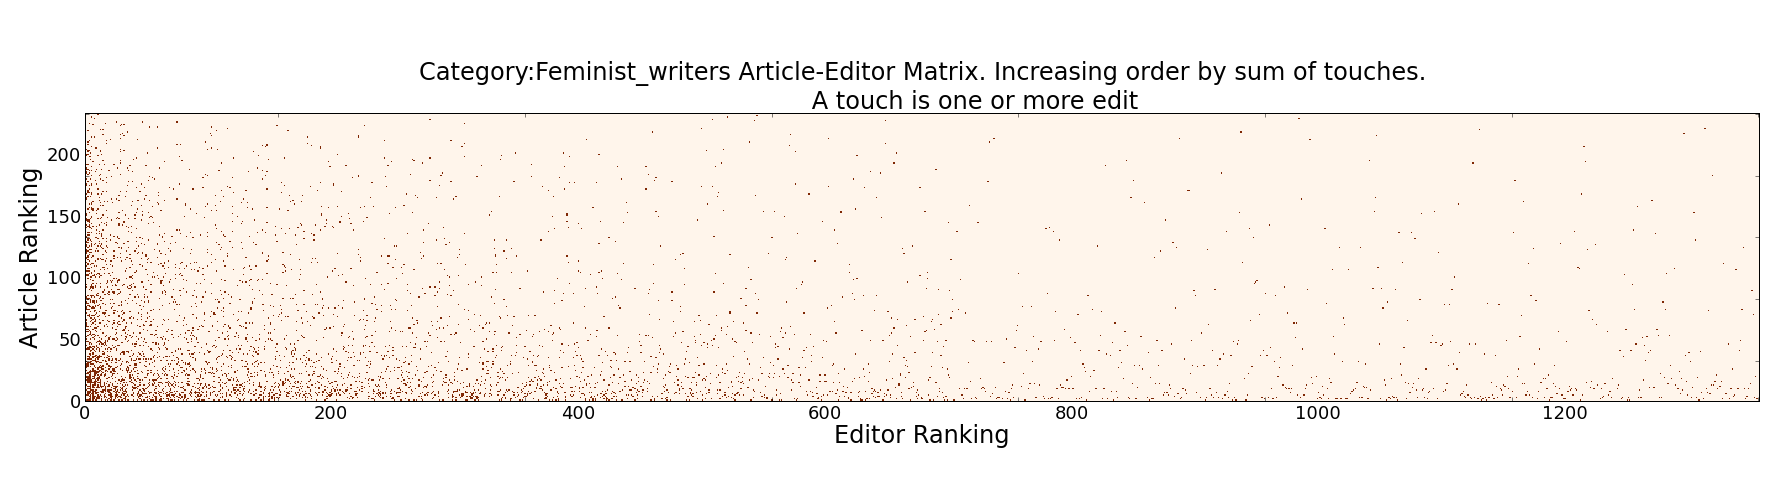
\includegraphics[width=2.0\columnwidth]{../Figures/Category_Feminist_writerstriangle_matrix_corrected.png}
\caption{Typical $\mathbf{\mathit{M_{ea}}}$ matrix for a Wikipedia category (here, {\it Feminist Writers}) ordered on both dimensions by descending order of number of articles modified by an editor (horizontal axis) and of number editors who have modified an article (vertical axis). The structure of $\mathbf{\mathit{M_{ea}}}$ is triangular and shows that some editors have a pervasive activity over articles, while most editors edit only a few. Similarly, some articles receive widespread attention by editors, while most articles are modified only by a few editors.}
\label{fig:triangle}
\end{figure*}

Given $M_{ea}$, the simplest, and arguably naive, way to assess the contribution value (i.e., the {\it expertise} thereafter) of an editor is obtained by summing the number of articles ever edited out of all articles in a category. Similarly, a simple {\it quality} measure for an article is the sum of editors who have ever modified it, following the famous adage on open source development: ``Given enough eyeballs, all bugs are shallow" \cite{raymond1999}. These crude expertise and quality metrics for editors and articles, respectively  given by,

\begin{equation}
\begin{cases}
 w_{e}^{(0)} = \sum_{a=1}^{N_{a}} M_{ea} \equiv k_e\\[7pt]
 w_{a}^{(0)} = \sum_{e=1}^{N_{e}} M_{ea} \equiv k_a
\end{cases}
\label{HHinit}
\end{equation}

are the zero\textsuperscript{th} order of our algorithm. They are the initial step of the {\it method of reflections} proposed by Hidalgo et al., which derives the value of producing entities (i.e., editors) from products (i.e., articles), and {\it vice versa} \cite{hidalgo2007,hidalgo2009}. To help capture the intuition behind the method of reflections for open collaboration, we walk through the first and second iterations:

\begin{itemize}
  \item {\bf 1\textsuperscript{st} order iteration,}  
  \begin{itemize}
  \item {\bf Articles}: if an article has been edited by higher expertise editors, it is of higher quality. That is, quality is a function of expertise calculated from zero\textsuperscript{th} iteration expertise scores.
  \item {\bf Editors}: conversely, if an editor has contributed to higher quality articles, her expertise is higher. That is, expertise is a function of quality calculated from zero\textsuperscript{th} iteration quality scores.
  \end{itemize}
  \item {\bf 2\textsuperscript{nd} order iteration,}
    \begin{itemize}
  \item {\bf Articles}: if an article has been edited by higher expertise editors who have edited higher value articles, which in turn have been edited by higher expertise contributors, the article quality is higher. That is, quality is a function of expertise calculated from 1\textsuperscript{st} iteration expertise scores.
  \item {\bf Editors}: conversely, if an editor has edited higher quality articles, which have been edited by better editors who have edited higher quality articles, then expertise is higher. That is, expertise is a function of quality calculated from 1\textsuperscript{st} iteration quality scores.
  \end{itemize}
 \item {\bf And so on, recursively.}\\
\end{itemize}

Although interpretation is difficult past the very first iteration steps, at each iteration, the algorithm incorporates additional information on the quality of the articles and expertise of editor from the neighboring nodes in the bi-partite network. The higher order iterations 
%of the method of reflections are written as,
%
%\begin{equation}
%\begin{cases}
% u_{e}^{(n+1)} = \frac{1}{k_{e}}\sum_{a=1}^{N_{a}} M_{ea} \, u_{a}^{n}\\[7pt]
% u_{a}^{(n+1)} = \frac{1}{k_{a}}\sum_{e=1}^{N_{e}} M _{ea}\, u_{e}^{n}\\
%\end{cases}
%\label{HHhigher}
%\end{equation}
%
% variable weights to the scores from the previous iteration
can be modeled as a Markov process of random walkers on a bi-partite network, jumping with some probability from one node type to another node type \cite{caldarelli2012network}. A schematic representation of the random walk process on a bi-partite network is depicted in Figure \ref{fig:jumpers}. The intuition is the following: a random walker jumps with some probability from an editor to a given article (i.e., the editor's expertise is positively influenced by the article's quality), and with another probability from an article to a given editor (i.e. the value of the article is positively by the editor's expertise). The binary matrix $M_{ea}$ determines whether a jump between each pair of nodes is possible: if two nodes $e$ and $a$ are not directly connected ($M_{ea} = 0$), the transition probability is 0. Conceptually, the {\it bi-partite network random walker} model is an extension of the single node type (i.e. Web pages) {\it Page Rank} Google search algorithm \cite{page1999pagerank,kleinberg1999} to two types of nodes.

\begin{figure}[!t]
\centering
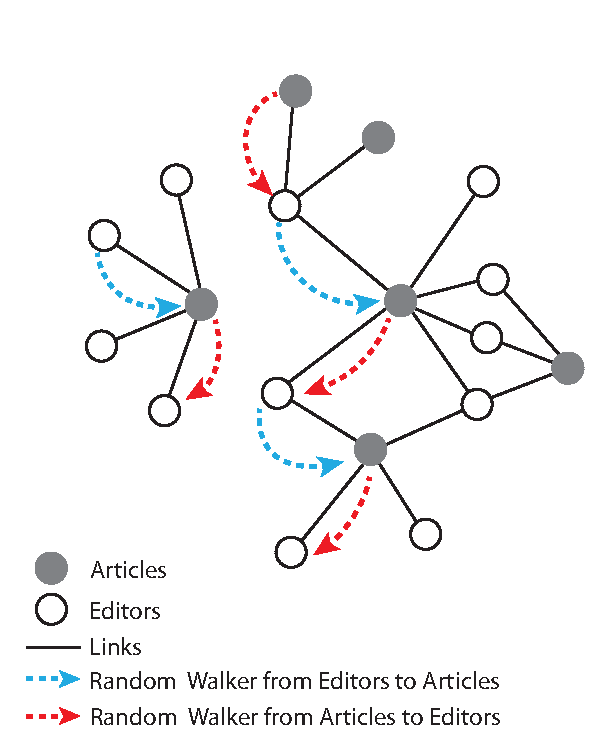
\includegraphics[width=0.7\columnwidth]{../Figures/bi-partite_net.eps}
\caption{Representation of random walkers jumping from editors to articles (red dotted arrows) and from articles to editors (blue dotted arrows). The intuition is the following: a random walker jumps with some probability from an editor to a given article (i.e., the editor's expertise is positively influenced by the article's quality), and with another probability from an article to a given editor (i.e., the value of the article positively influences the editor's expertise).}
\label{fig:jumpers}
\end{figure}

%According to  Caldarelli et al. \cite{caldarelli2012network}, we reformulate the method of reflections to account for jumps of the random walker on the bi-partite network of editors and articles. 
We call $w^{(n)}_e$ the expertise of an editor and $w^{(n)}_a$ the quality of an article at the $n^{th}$ iteration, and we define the following Markov process on the bi-partite network of collaboration, 

\begin{equation}
\begin{cases}
w^{(n+1)}_e (\alpha,\beta) = \sum_{a=1}^{N_a}  G_{ea}(\beta) \,w^{(n)}_a (\alpha,\beta)\\[7pt]
w^{(n+1)}_a (\alpha,\beta) = \sum_{e=1}^{N_e}  G_{ae}(\alpha) \, w^{(n)}_e (\alpha,\beta)\\
\end{cases}
\label{random_walker}
\end{equation}

with $G_{ea}$ the probability  to jump from article $a$ to editor $e$ in a single step, and the probability $G_{ae}$ to jump from editor $e$ to article $a$ also in a single step. These transition probabilities are given by,

\begin{equation}
\begin{cases}
G_{ea}(\beta) = \frac{M_{ea} k_{e}^{-\beta}}{\sum_{e' = 1}^{N_e} M_{e'a} k_{e'}^{-\beta}}\\[10pt]
G_{ae}(\alpha) = \frac{M_{ea} k_{a}^{-\alpha}}{\sum_{a' = 1}^{N_a} M_{ea'} k_{a'}^{-\alpha}}.\\
 \end{cases}
\end{equation}

The transition matrices $G_{ea}(\beta)$ and $G_{ae}(\alpha)$ depend only on the initial conditions: the binary matrix $M_{ea}$, as well as $k_e$ and $k_a$ given by (\ref{HHinit}), and are controlled only by parameters $\alpha$ and $\beta$.  We shall therefore explain only how $\beta$ influences the probability to jump from an article to an editor (i.e. the value of the article positively influences the editor's expertise). For $\beta = 0$, we recover the zero\textsuperscript{th} order iteration (\ref{HHinit}). For $\beta > 0$, the probability to jump from article $a$ to editor $e$ is a power law function $\sim 1/k_{e}^{~\beta}$ of the sum of articles $k_{e}$  modified by editor $e$. Hence, the larger $k_{e}$, the lower the probability to jump from $a$ to $e$ relative to other editors. On the contrary, if $\beta < 0$ the probability to jump from an article to an editor is a positive function of the sum of articles modified by the editor. For $-1 < \beta < 0$, the function is concave, while for $\beta < -1$, the function is convex, which means that the more articles have been edited by the editor, the even more the positive influence on articles. In a nutshell, $\beta$ relates the amount of articles edited on the overall editor's expertise. %which in turn has an influence on each edited article (along with the influence of other editors).
If $\beta \gg 0$, the positive influence of the number of contributed articles on the editor's expertise decreases. If $\beta$ close to $0$, the number of contributed articles increases linearly the editor's expertise. The same considerations hold for $\alpha$ and the probability $G_{ae}(\alpha)$ to jump from an editor to an article (i.e. the expertise of the editor positively influences the quality of an article).

%After each iteration, we have expertise and quality scores, which allow for the ranking of editors and articles respectively. When the rankings for both editors and articles do not change in two successive iterations we consider that the {\it bi-partite network random walker} model has converged. We have verified that the method converges on all our 12 Wikipedia categories.  
Figure \ref{fig:convergence} shows the evolution of expertise $w_e$ ranked among editors having contributed to articles in the {\it Feminist Writers} category on Wikipedia for the set of control parameters $(\alpha,\beta) =(0, 0.72)$. We can see how the algorithm progressively ranks editors: some editors with initial low rank (i.e. with few articles edited), get a higher rank as more information is incorporated from neighboring nodes as the number of iterations increases. In that case ($\beta >0$), higher ranked editors have edited and contributed to fewer, but higher quality articles (i.e. articles edited by more editors who have edited less articles). Similarly, some initially high ranked editors, gradually drop in the ranking. They have edited many, but lower quality articles. 

\begin{figure}[!t]
\centering
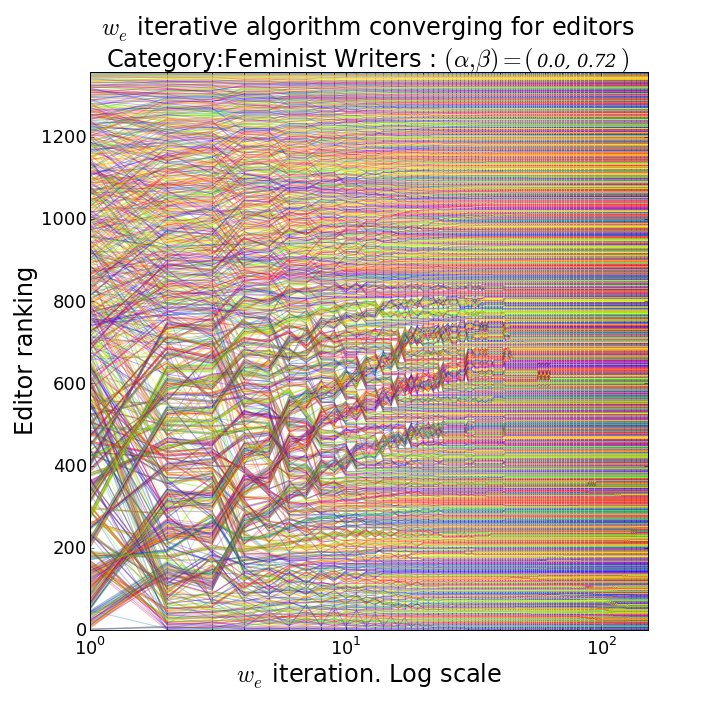
\includegraphics[width=0.9\columnwidth]{../Figures/fem_editors_iter_converge.png}
\caption{Convergence of the ranked expertise $w_e$ of editors having contributed to articles in the Feminist Writers category on Wikipedia for arbitrary control parameters: $\mathbf{(\alpha,\beta) =(0, 0.72)}$. Starting from the sum of contributed articles as the initial step, we can see how the algorithm progressively ranks editors: some editors with initial lowest rank, i.e., with few articles edited, get a higher rank as the number of iterations increases. Similarly, some initially high ranked editors, gradually drop in the ranking. In the case {\it Feminist Writers}, the algorithm converges after $\mathbf{64}$ iterations.}
\label{fig:convergence}
\end{figure}

Upon calibration of the bi-partite random walker model with ground-truth metrics of article quality and editor expertise, the parameters $\alpha$ and $\beta$  directly inform how coordination generates value (i.e. more articles edited by more editors brings value), or on the contrary, if value is created by small clusters of highly experienced editors. This latter scenario implies less coordination among large crowds of contributors.

% describe how editors and articles influence each other at the level of the whole bi-partite collaboration network.
%\textcolor{red}{We cannot calibrate and test because each category is different}
%Whenever calibration shows that the evolution of $\alpha$ and $\beta$ can be predicted, then editor expertise and article quality can also be predicted up to statistical errors. 
%Here, we explain the calibration steps for$\alpha$ and $\beta$ and how the control parameters inform on the structure of value creation in open collaboration. We also document the evolution of these parameters as Wikipedia categories get increasingly enriched with new contributions.
%A property of this algorithm, is that with the following balance condition,
%
%\begin{equation}
%\mathbf{G}_{ae} \mathbf{w}^*_e = \mathbf{G}_{ea} \mathbf{w}^*_a
%\end{equation}
%
%which can be rewritten as,
%
%\begin{equation}
%\begin{cases}
%\mathbf{w}^{*}_{e} \sim \mathbf{k}^{1-\beta}_{e} \langle \mathbf{k}_{a}^{-\alpha}\rangle_e \\
%\mathbf{w}^{*}_{a} \sim \mathbf{k}^{1-\alpha}_{a} \langle \mathbf{k}_{e}^{-\beta}\rangle_a
%\end{cases} \label{eqsim}
%\end{equation}
%
%it is the analytical formulation we use onwards. It is important to note a crucial difference in the way we apply the weighted random walk model in the case of open collaboration compared to the countries-products problem. In \cite{caldarelli2012network}, $w^*_p$ is a measure of ubiquity (i.e. dis-quality) because many countries can sell the product, while here $w^*_a$ is also a measure of ubiquity in the sense that many editors have modified the article. In the case of open collaboration, $w^*_a$ is a measure of quality.
